%ब
\section{Apache Cassandra} \label{s:Background-Cassandra}

Cassandra is a distributed data storage system initially developed by Facebook
for satisfying the needs of large web applications that handle large
volumes of data (\todo{cite BOOK}). 
Its development is now undertaken by Apache  and is being used by
many large web applications and large organisations like Facebook,  Twitter, 
Cisco,  Digg,  Reddit among others (\todo{Gunda,  2010}). 

Cassandra is based on the column-oriented key value data model and stores data
as columns,  super columns,  column families and keyspaces all of which are
explained in Section~\ref{s:key-value-data-model}. It is run as a single Java
process run on a machine and is designed to work  across different machines and
across multiple data centers,  even data centers that are geographically
distributed(\todo{ BOOK}).  The details of such a distributed nature is
abstracted from  the user such that everything appears stored on a single
machine.  This distributed nature makes Cassandra better utilised when it is run
on multiple machines that are configured to operate together and run as a single
cluster  (\todo{Perham,  2010a,  BOOK}).  These machines in the cluster form a ring
of nodes,  where nodes are connected to each other and each node is aware of all
their peers in the cluster (Figure~\ref{f:cassandra-cluster})). 


\begin{figure}[h] \centering 
	% \includegraphics[width=5cm,    height=5cm]{.  /figure/random.  jpg}
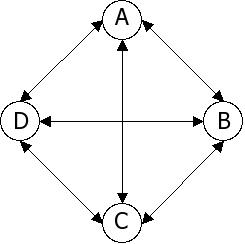
\includegraphics[width=.3\textwidth]{./figure/Cassandra/Cassandra-cluster.png}
	\caption{A cluster of nodes in Cassandra}\label{f:cassandra-cluster}
\end{figure}

The nodes in a cluster communicate with each other to send their state
information at regular time intervals,  so that other nodes in the ring can know
their status (\todo{cite Cassandra paper}).  This helps in failure detection in
Cassandra since if a node is not active,  it fails to send or respond to messages
from other active nodes and in this way the rest of the nodes  know of its
inactive state.  In the event of a node failure,  another active node  performs
the operations in order to ensure that  operations  sent to the failed node are
not lost (\todo{cite Cassandra papers}). 

In such a cluster,  every node applies the same architectural features
fundamental to Cassandra,  namely,  load balancing,  replicating
and partitioning data,  failure detection mechanisms among others.  Some of the
key architectural concepts of Cassandra are explained next. 

% Distributed system are prone to conflicts as many users could be issuing
% requests on data items from any of the nodes.  Any distributed system should
% carefully consider conflict resolution and adopt design approaches which would
% resolve such conflicts efficiently.  Conflicts arise either at read or write
% operations. 
% The design approach should either make the system resolve such conflicts either
% during one of these operations,  deciding the system be either readable at all
% times or writable.  Cassandra optimises its performance by adopting the design
% approach of resolving conflicts during read operations,  making Cassandra always
% writable. 



\subsection{Cassandra Architecture} \label{ss:Background-Cassandra-Archi}
Cassandra adopts a lot of its architectural concepts from other popular
distributed key-value data storage systems on the cloud,  like Google's Bigtable
and Amazon's Dynamo (\todo{cite}).  Overtime these adopted concepts evolved and
developed new features,  some of which became specific to Cassandra's
architecture.  These architectural concepts gave
Cassandra its popular features like elastic scalability,  fault tolerance,  high
availability and high performance. 
% Cassandra's architecture involves many sophisticated and complex theoretical
% as well as mathematical concepts,  
Following are some of the key architectural concepts of Cassandra. 
% Discussing every concept is beyond the scope of this research. 

\begin{description}

\item[Peer-Peer Distribution Model:] 
% Generally,  in traditional distributed
% \acp{DBMS},  nodes in a cluster are configured to have different
% responsibilities and roles where some or one of the nodes is a master and others
% are slaves.  Such a centralised configuration improves reading data,  as data can
% be read from any of the slave nodes,  but write requests are always sent to the
% master node.  This model thus puts a lot of additional load on the master and
% also is prone to failure if the single master node is offline.  However, 
Cassandra is a decentralised system,  where all the nodes are considered equal
or identical (i. e.  nodes are peers) in sharing responsibilities and performing
operations,  without any  master or slave nodes (\todo{cite book}). 
This model provides high data availability since failure
of a node does not affect the service of the cluster,  because other
nodes can carry out the same operation. 
% Moreover,  when new nodes are added to a cluster there is no additional task of
% delegating responsibilities or roles since all the nodes have the same
% responsibilites. 

% The nodes in a cluster communicate with each other to send their state
% information at regular time intervals,  so that other nodes in the ring can know
% their status (\todo{cite Cassandra paper}).  This helps in failure detection in
% Cassandra since if a node is not active it fails to send or respond to  messages
% from other active nodes and in this way the rest of the nodes  know of its
% inactive state.  In the event of a node failure,  another active node  performs
% the operations in order to ensure that  operations that were sent to a failed
% node are not lost (\todo{cite Cassandra papers}). 
% The recepient node  creates a small hint message with the information about
% the operation so that it can give the hint to the failed node once it is
% alive again and this feature is called hinted handoff. 

\item[Partitioning Data:] Cassandra partitions data between the nodes in a
cluster  so that data items from overloaded or failed nodes are
assigned to other nodes or new nodes.  For this,  Cassandra uses consistent
hashing where data items are hashed on its key and assigned  to the node that
has its  token (i. e.  position in the ring) larger than this hashed value
(\todo{cite book}). 

% used by Amazon's Dynamo to partition data over the nodes. (\todo{DeCandia et
% al. (2007)}). 

% \begin{figure}[h] \centering %\includegraphics[width=5cm,    height=5cm]{. 
% /figure/random.  jpg}
% 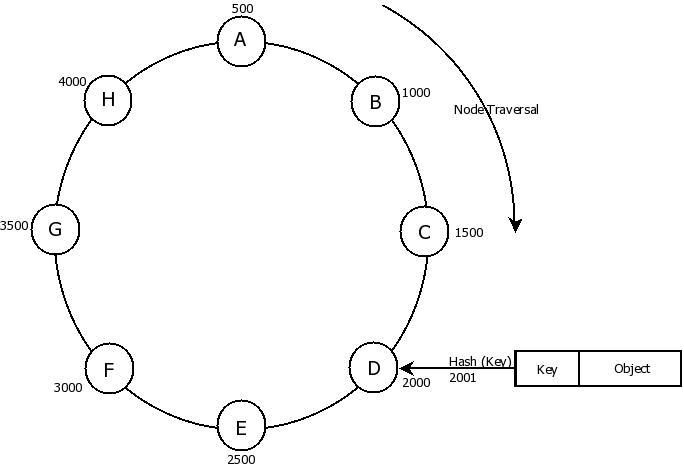
\includegraphics[width=. 6\textwidth]{. /figure/Cassandra/Consistent-hashing-Cassandra. png}
% \caption{Consistent hashing in Cassandra}\label{f:consistent hashing}
% \end{figure}

Partitioning data makes Cassandra elastically scalable since load is balanced
and distributed in the cluster  irrespective of addition or removal of nodes
(\todo{cite Book,  most Cassandra papers}). It also improves load balancing of a
cluster since workload is distributed  without affecting the performance of the
whole cluster. 
% Additionally,  in Cassandra better performing nodes are assigned multiple
% points in the ring,  making them virtual nodes and these nodes are assigned
% workloads from failed nodes or overloaded nodes. 

\item  [Replication strategy]: In order to ensure high data availability
irrespective of failures,  Cassandra uses a replication strategy where every data
item is replicated across a number of nodes specified by the user.  Users can set
the level of replication they  prefer,  by setting the replication factor to the
number of nodes they  prefer to use for replication(\todo{cite Book,  most
Cassandra papers}).  In other words,  replication factor tells the cluster how
many copies to save of a single data item.  Setting the replication factor to a
large number would help in higher consistency of data items,  but replicating
data items to a large number of nodes each time there is an operation on it,  
can adversely affect the performance. 

Thus,  once data items are partitioned and assigned to a node,  these are
replicated onto other nodes and a list of the nodes responsible for storing the
data items are maintained.  This way every node in the cluster knows which nodes
are responsible for a data item (\todo{cite Book,  most Cassandra papers}). 
Such a replication strategy makes data highly available  since data items can
be accessed from any node in a cluster regardless of node failures.  
% Since all
% the nodes  know which peer node is responsible for a data item,  
% routing requests to the correct nodes. 



\item [Eventual Consistency]:
% As mentioned previously,  Cassandra opts for '\texttt{A}' and '\texttt{P}' of
% the CAP theorem and allows users to determine the level of consistency they 
% prefer.  This consistency level tells the cluster how many replicas should
% acknowledge operations done on them,  for the replicas to be considered
% consistent and up to date.  Low consistency levels are considered better for
% performance as higher consistency levels involve more time since nodes have to
% wait to receive acknowledgements from more replicas. 
% Letting the users decide the consistency level and replication factor means
% the tradeoff between consostency and performnace is detemined by the users. 
Cassandra uses the eventual consistency model where every replica agrees to the
most recent value after a certain point in time and allows updates to be
propagated to all the replicas asynchronously  (\todo{Henry,  2008}). Thus,  all
replicas would be consistent eventually after a certain period of time, 
generally a small number of milliseconds \todo{cite book}. 
This is unlike strict consistency models in traditional \acp{DBMS} run on single
nodes,  where a read operation always returns the most update values.  However,  in
distributed systems like Cassandra,  more machines are used concurrently by many
users leading to various conflicts,  which makes a weaker form of consistency
like eventual consistency  ideal (\todo{cite BOOK and marked papers}). 

\end{description}
The architectural concepts form the foundation of Cassandra,   providing it
with BASE properties and many important features like high data availability,
failure management, fault tolerance and scalability among others.  These
concepts and features of Cassandra influence its read and write operations,
which are designed to implement these concepts and enhance the features of
Cassandra.  The read and write operations are briefly explained in the following
section.

\subsection{Write and Read Operations}
\label{ss:Background-Cassandra-Operations} 
In order to write data into Cassandra column families,  a write request is sent
to a random node in the cluster,  which acts as the proxy node and replicates the
data in the cluster. 
The number of nodes on which data should be replicated can be set by the users
and these  nodes can be in the same data centre and 
other data centres.  These nodes would act as proxies when they receive
write requests and  make data recoverable from other nodes(\todo{Perham, 
2010a}). 
		

When a read request is issued to a node,  it acts as a proxy node and forwards
the request to all the other nodes in the cluster.
These nodes return their copy of the data item to the proxy node and the proxy
node  checks the versions of the replicas and sends the latest replica to the
user  (\todo{Perham,  2010b}).   If the replicas received from a node are not
consistent with other replicas, a read repair is performed on the node
with the outdated replicas.  This means that the nodes with outdated replicas
are sent a write operation with the latest data.
Thus,  data consistency is maintained whenever conflicting versions of data
items are found.


These key architectural concepts and operations of Cassandra are designed to
make it a highly available and scalable \ac{DBMS},  with many features like data
partitioning,  fault tolerance,  replication and others to make it suitable for
cloud environments.   
This \ac{DBMS} is used to implement the four solutions
designed to impose referential integrity validations in cloud \ac{NoSQL}
\acp{DBMS}.  The design of these solutions  and the approaches used to
implement such validations are explained in the following chapter. 
